\iffalse
\bibliography{reference/refs}
\fi


\chapter{Face De-Identification in Still Images}
\label{chap:FDimages}

With the quick development of Internet and web applications, 
people are willing to publish self pictures. Furthermore, 
most of the pictures are allowed to access without permissions. 
Thus the problem of privacy protection must be considered.
This chapter introduces our face de-identification algorithms 
in still images on tensor CP decomposition. 

Tensor analysis, also known as multilinear algebra, makes 
the assumption that images are formed as a result of multiple 
factors. Previous researches indicate that it is possible to
alter one factor remaining other factors constant\cite{VasilescuT03}. 
In this chapter, an overview of the algorithm is firstly 
described and then other procedures are illustrated step by step. 
At last, related experiments would prove the effevtiveness
of the proposed algorithm.

\section{Algorithm Overview}
This section describes the overview of the proposed algorithm.
To abstract the method in one word, a face image is decomposed
into multiple factors and only the privacy related ones are
altered to reconstruct a new face image. This method has advantages
in processing the dataset with multiple types of data utilities.
The whole procedure of our de-identification algorithm is 
illustrated in Fig. \ref{fig:diagram}. 

\begin{figure}[!htb]
    \centering
    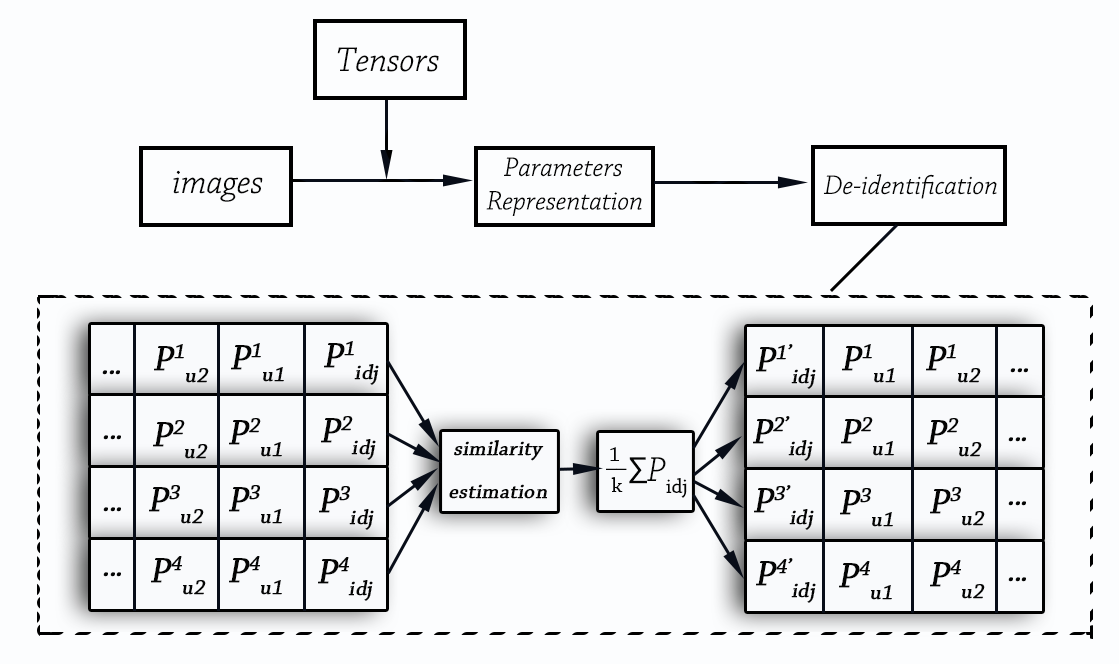
\includegraphics[scale=0.7]{figure/overflow}
    \caption{Overview of the proposed algorithm. Dashed box is the de-identification process. Each row 
    in the dashed box is one parameters representation of a image. $P_{idj}$ is the {\it identity}
    parameters. $P_{u1},P_{u2},...$ are the {\it utility} parameters.}
    \label{fig:diagram}
\end{figure}

Firstly, a tensor of face images is pre-constructed. As stated before,
we arrange the images with different types of data utilites in some order.
The purpose is to extract the common features between these images.

Secondly, we project a face image, $img$,
into the pre-constructed tensor to get multiple types of parameters.
However, we can only get a set of parameters that is a combination
of the individual parameters for dimensions. Therefore, we should
then decompose the whole parameters into multiple diemensions. One
of them is $identity$ parameters.

Finally, we select $k$ other images whose {\it identity} parameters 
are the farthest from $img$ and other types of parameters most 
closest to $img$. The final de-identified result is the face image 
which is reconstructed using altered {\it identity} and other 
original parameters.

\section{Tensor Construction}

First of all, we pre-construct a tensor of face images according to
the required data utilities. It is a container for all image data.
A tensor is defined as multiple dimentional array or $n$-mode array. 
For example, a vector is $1$-mode tensor and
a matrix is $2$-mode tensor. The $n$-mode tensor ($n>2$) is called 
the higher-order tensor. 

According to the theory of PCA, each item of a set of $1$-mode data 
could be represented by the specific parameters and a basis vector. 
Inferred from that, multiple array has the same property for each
dimension. In PCA implementation, each data item is represented by
a vector and all data are formed as a matrix at last. Therefore, 
the images with the same data utility are placed into one dimension 
in the higher-order tensor so that the common features could be 
extracted. 

To explain more clearly, an example of tensor construction is shown in
Figure \ref{fig:tensor}. It contains three types of data utility:
identities, expressions and poses. Each image is represented as
a vector, and the images are placed along different axis based 
on the various data utilities. The image tensor with three types of factors
is then illustrated in a three dimensional coordinate. When there are
more types of the data utility, we could add more dimensions in the coordinate
for tensor representation.

\begin{figure}[!htb]
    \centering
	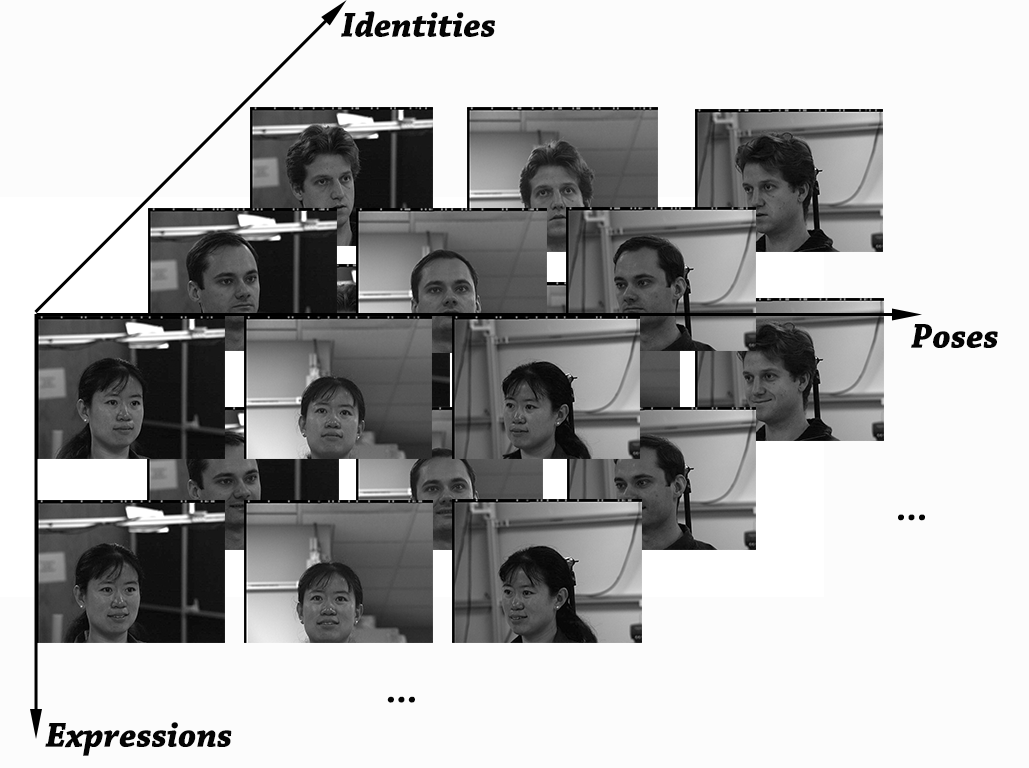
\includegraphics[scale = 0.75]{figure/tensor.png}
    \caption{Tensor Construction. Each axis is one dimension of the tensor 
    and each dimension in the tensors represents one factor of the images.}
    \label{fig:tensor}
\end{figure}

Shown as the above figure, all the images along $Poses$ axis have
the same $identity$ and $expression$, but different $poses$. Similarly,
the images along $Identities$ axis are with the same $pose$ and
$expression$, but different $identity$. Therefore, the final tensor is
a $3$-mode array, $\mathcal{A} \in R^{identity \times expression \times pose}$. 


  \section{Image Projection}
  The next step is to project an image into the tensor to get the corresponding
  parameters. The conventional tensor decomposition theory such as HOSVD 
  \cite{Lathauwer00} is possible to extract parameters of one dimension by 
  defining a basis tensor. However, it is not possible to get the parameters 
  for each dimension. Hence, this section gets a set of parameters for an image 
  and then decomposes it into multiple factors. 

  As stated before, a 2D face image, $img$, could be represented by a set of
  parameters and a tensor. The parameters are a mixture result of multiple factors. 
  Suppose the number of these factors is $n$, we could construct a mode-$(n+1)$ tensor
  using proper number of face images, represented as 
  $\mathcal{I} \in R^{i_1 \times i_2 \times ... \times i_n \times i_{data}}$.  
  The $i_{data}$ dimension contains data from face images. 
  For example, if the images are separated into three categories: $identity,expression,pose$, we can
  build a tensor as $\mathcal{A} \in R^{identity \times expression \times pose \times pixel}$. The pixels
  are just the data from face images. With this tensor, each $img$ could be represented by a set of
  parameters. 

  In the previous researches \cite{VasilescuT03,TPAMI09} and many practical examples such as 
  image relighting \cite{lin05} and expression transfer \cite{Macedo06}, a tensor is usually 
  decomposed by Higher-Order 
  Singular Value Decomposition (HOSVD) ~\cite{Lathauwer00}:
    \begin{equation}
      \begin{aligned}
        \mathcal{I} = \mathcal{Z}_{core} \times_1  U_1  \times_2 U_2 ... \times_n U_n \times_{n+1} U_{data}, 
      \end{aligned}
    \end{equation}
    where $\mathcal{Z}_{core}$, called {\it core tensor}, is the same size as $\mathcal{I}$. One of the 
    matrices in $U_1,U_2,...,U_n,U_{data}$, $U_i$ is the left part in SVD results of corresponding 
    mode-$i$ flattening of $\mathcal{I}$.

  Each $img$ in $\mathcal{I}$ could be described as the HOSVD decomposition and a set of vector parameters, 
  $({\bf c_1,c_2,...,c_n})$. Therefore, each $img$ is written
  as:
    \begin{equation}
    \label{equ:cp_decompose}
      \begin{aligned}
        img & = \mathcal{Z}_{core} \times_1  ({\bf c_1^T}*U_1) ... \times_n ({\bf c_n^T}*U_n) \times_{n+1} U_{data} \\
          & = (\mathcal{Z}_{core} \times_1 U_1 ... \times_n U_n \times_{n+1} U_{data}) \times_1 {\bf c_1^T ... \times_n c_n^T} \\
          & = \mathcal{I} \times_1 \underbrace{ {\bf c_1^T} \times_2 {\bf c_2^T} ... \times_n {\bf c_n^T} }_{ {\bf c_{para} = c_1 \otimes c_2 ... \otimes c_n} }\\
          & = I(data) * {\bf c_{para}}, 
      \end{aligned}
    \end{equation}
    where $I(data)$ is the flattening matrix of $\mathcal{I}$ in mode-$(n+1)$, ${\bf c_{para}}$ is the 
    Kronecker product of all kinds of parameters. 

    Through the above statement, we can naturally conclude that the projection of a face image into the 
    inverse space of a pre-defined image set is the representation parameters for this image in the set. 
    Inferred from the Equ. \ref{equ:cp_decompose}, an image $img$ is the result of $I(data)$ and 
    ${\bf c_{para}}$. Suppose the size of $I(data) \in R^{w*h}$, $img$ is unique only when $w \geq h$. 
    Therefore, {\it K-Nearest Equation Construction} strategy ~\cite{lin05} is used to guarantee the constraint. 
    Since $I(data)$ is not promised to be a square matrix, ${\bf c_{para}}$ is represented in mathematics as:
    \begin{equation}
      \begin{aligned}
        {\bf c_{para}} & = I(data)^{-1} * img\\
                 & = I(data)^T * (I(data)*I(data)^T)^{-1} * img.
      \end{aligned}
    \end{equation}  

    \section{Parameters Decomposition}

    The previous section shows how to project one image into a data space composing 
    of multiple types of images. Each image is represented as a set of parameters.
    So far, the previous ${\bf (c_1,c_2,...,c_n) }$ are all assumed to be known, but we can only get their
    Kronecker product, ${\bf c_{para} }$ which can be seen as the parameters of a face image. Next step is to
    decompose the entire parameters into different types. It has been tried to get best vector parameters in 
    HOSVD using optimization algorithms \cite{lin05}. The method is similar to rank-$1$ approximation of 
    ${\bf c_{para} }$ based on tensor CP decomposition, which is used in \cite{TPAMI09} as {\it continuous variation 
    estimation}. However, the rank-$1$ approximation is easily converges to local optimization \cite{Lathauwer_rank}, 
    which would leads to low quality representation. We use rank-$r$ approximation of tensor CP decomposition
    to decompose the parameters here. 

    To decompose ${\bf c_{para} }$, it is firstly reshaped as a tensor $\mathcal{C} \in R^{i_1 \times i_2 
    \times ... \times i_n}$ which is the same size as $\mathcal{I}$ in previous $n$ dimensions. According
    to tensor CP decomposition, any 
    tensor can be represented as a sum of tensor product by vectors \cite{Lathauwer_rank}, shown as 
    (\ref{equ:cp}).

    \begin{equation}
      \label{equ:cp_no}
      \begin{aligned}
        \mathcal{C} = \sum_{i=1}^{r}\lambda_i * {\bf c_1^i} \circ {\bf c_2^i} \circ...\circ {\bf c_n^i},  
      \end{aligned}
    \end{equation}
    where $\circ$ indicates tensor product. It indicates that $\mathcal{C}$ can be decomposed into $r$ components 
    of tensor product by $n$ vectors.

    The $r$ value is undetermined. We can pre-define a value $threshold$ (e.g. 0.01). The determiend $r$
    ($r \geq 1$)should be the first value that makes the deviation between original parameters and reconstructed 
    tensor less than this value.
    In mathematics, it could be represented as:
    
    \begin{equation}
      \begin{aligned}
         \ \ \| \sum_{i=1}^{r}\lambda_i {\bf c_{1}^i} \circ {\bf c_{2}^i} \circ ... \circ {\bf c_{n}^i} - \mathcal{C} \|_r \leq threshold.
      \end{aligned}
    \end{equation}

    After the determination of $r$, one image, {\it img}, is a explained as a combination of $r$ subimages. Illustrated
    as (\ref{equ:phy}), each of these subimages is formed
    as a result of multiple factors. 
    \begin{equation}
      \label{equ:phy}
      \begin{aligned}
        img & = \mathcal{I} \times \mathcal{C} \\  
          & = \mathcal{I} \times (\sum_{i=1}^{r} \lambda_i * {\bf c_1^i} \circ {\bf c_2^i} \circ...\circ {\bf c_n^i}) \\
          & = \sum_{i=1}^{r} \lambda_i * \mathcal{I} \times_1 {\bf c_1^i} \times_2 {\bf c_2^i} ... \times_n {\bf c_n^i}, 
      \end{aligned}
    \end{equation}

    Compared with the other tensor decomposition methods, the CP decomposition approaches
    have advantage in processing the images that never appear in the pre-constructed
    tensor. Using the ALS approximation method, the parameters for each dimension is
    restored properly. Thus, our method enlarges the representation ability of the 
    pre-constructed tensor.

    \section{De-Identification}
    It has been shown how to represent a face image by different types of parameters in previous sections. 
    Next step is to de-identify a target with some selected images. The selection method is important. For
    example, $k$-same framework fails to protect privacy in a dataset with multiple images for each person
    because it has to 
    choose the closest neighbors for each image. The decomposition of face images would overcome that
    problem by selecting images whose {\it identity} parameters are the farthest from the target and the 
    other {\it utility} parameters are closest to that target.

    As stated in Eq. (\ref{equ:phy}), a face image could be represented by $r$ subimages with each one
    of them being the confluence of multiple factors. One of these factors is {\it identity}. Since the
    order is trivial, we assume the ${\bf c_1}$ is the {\it identity} parameters, so
    $\mathcal{C} = \sum_{i=1}^{r}\lambda_i * {\bf c_{idj}^i} \circ {\bf c_2^i} \circ...\circ {\bf c_n^i}$.
    The {\it identity} parameters are represented by ${\bf c_{idj} }$ in the following text.

    Suppose there are two images $img_1$ and $img_2$ and their parameters are ${\bf c_{img_1} \in 
    \sum_{i=1}^{r_1}c_{idj\_1}^i \circ c_{2\_1} ... \circ c_{n\_1} }$ and ${\bf c_{img_2} \in 
    \sum_{i=1}^{r_2}c_{idj\_2}^i \circ c_{2\_2} ... \circ c_{n\_2} }$. The similarity score 
    between these two images is:
    \begin{equation}
    \label{equ:similar}
      \begin{aligned}
        similarity = \ \ \| \sum_{i=1}^{r_1}\lambda_1^i*{\bf c_{idj\_1}^i }  - \sum_{i=1}^{r_2}\lambda_2^i* {\bf c_{idj\_2}^i }\|  - \\
                     \sum_{j=2}^{n}\ \ \|  \sum_{i=1}^{r_1}\lambda_1^i*{\bf c_{j\_1}^i}  - \sum_{i=1}^{r_2}\lambda_2^i*{\bf c_{j\_2}^i }\|.
      \end{aligned}
    \end{equation}

    Despite of the complexity of the $similarity$ euqation Eq. (\ref{equ:similar}), it is summarized as 
    testing the similarity by using the Euclidean distance between images in quantization.
    Specifically, we use the parameters in $identity$ minus the sum of parameters in other $utility$ dimensions.
    For a target image, we can find out the images whose $identity$ farthest from it and the other
    $utility$ parameters closest to it by picking out the images with largest $similarity$ scores to the target one.
    Compared to the $k$-same framework, our approach has the advantage in dividing the parameters
    into pirvacy related factors and non-privacy related ones. Hence the image classification is
    more accurate. 

    For a target image with {\it identity} parameters ${\bf c_{idj\_1}}$, we can find $(k-1)$ images according to
    (\ref{equ:similar}). The {\it identity} parameters are ${\bf c_{idj\_2},...,c_{idj\_k}}$. The de-identified result
    of the target iamge is:
    \begin{equation}
      \begin{aligned}
        result & = I_{(data)} * (\sum_{i=1}^{m} \lambda_i(\frac{1}{k}*\sum_{j=1}^k {\bf c_{idj\_j}^i} ) \circ {\bf c_{2}^i} \circ ... \circ {\bf c_{n}^i}).
      \end{aligned}
      \label{equ:compo}
    \end{equation}

    \section{Approach Summary}

    Based on a pre-constructed image tensor, a new image is firstly projected to
    the tensor for parameter representation. Then its parameter is decomposed into
    $identity$ factors and other data utility ones such as $pose$, $expression$. 
    At last, the de-identification process focuses only on $identity$ dimension. 

    The advantage of this approach is to break the limit of person specific dataset.
    Since the privacy related factors and the non-privacy related ones are separated,
    our approach picks the $identity$ part out and produces a new one 
    according to the $identity$ factors from other persons. Therefore, it allows that
    each person in the dataset could have multiple images. Furthermore, 
    the approach is flexible when more types of images are added dynamically.
    The pre-constructed tensor could be extended to meet the increasing images.

    To make the
    algorithm clearer, the following steps are listed to summarize the procedures.


    \medskip
      \noindent
        {\it Face De-identification in Images Based on Tensor CP Decomposition:}
        \begin{verbatim}
        1. Build a tensor according to the required utility
           types,
        2. Project a target image into the tensor to get
           an entire parameter vector,
        3. Decompose the parameter vector into multiple
           dimensions, one of which is identity,
        4. Select k images according to Eq. (7),
        5. De-identify the target image according to Eq. (8).
        \end{verbatim}
        %
      \noindent

      There are still some shortcomings for this approach. The pre-constructed tensor
      requires a completed dataset. Suppose a $3$-mode tensor would be constructed, three
      types of images are necessary for each item. If three kinds of factors are required,
      ($pose$ (left, frontal, right), $expression$ (smile, normal) and $identity$), each person
      should have 6 images to construct a tensor. It is not easy to get complete dataset.
      In practical, the missing value is replaced by the average of existed data 
      to solve this problem \cite{Feng12}. That is a useful research problem in the future.

%%%%%%%%%%%%%%%%%%%%%%%%%%%%%%%%%%%%%%%%%%%%%%%%%%%%%%%%%%%%%%%%%%%%%%%%%%%%%%%%%%%%%%%%%%%%%%%%%%%%%
%           
%%%%%%%%%%%%%%%%%%%%%%%%%%%%%%%%%%%%%%%%%%%%%%%%%%%%%%%%%%%%%%%%%%%%%%%%%%%%%%%%%%%%%%%%%%%%%%%%%%%%%
\section{Experiments and Results}

We conduct the experiments on CMU PIE database \cite{PIE01} and IMM database \cite{IMM04}. 
Sandia tensor toolbox \cite{TTB15} is used to analyze the tensor. The program is executed in 
Matlab R2014b. In this section, we show the de-identified images and automatic recognition
ratios, then explain the reasons why we use rank-$r$ approximation for parameters decomposition. 

\subsection{De-identified Images}
For CMU PIE database, a tensor is constructed based on three factors: {\it identity, pose, expression}.
Images from 20 subjects are chosen. Each one of them has 3 poses: frontal, left profile, right profile, 
and 2 expressions: normal and smile. All selected images are without glasses. The other images are 
for testing. 

Firstly, we use face landmarks detection algorithm from Dlib to get the shapes of all images, 
then warp the pixels within shape region to a mean shape. Similar as AAM, one image produces two kinds 
of data, shape and appearance. The shape remains unchange during de-identification for it influences
mainly on $poses$ rather than $identity$. Finally, the tensor model is built only on appearance data.
In this experiment, appearances are warped into a mean shape to form images as the size of $184*194$.
It would be time consuming if the appearance is formed as a $(184*194) \times 1$ vector. Therefore, 2D
appearance representation proposed in \cite{Feng12} is referenced to speed up the computation. Following
the procedures described in this chapter, we produce the comparison between original
images and de-identified ones as shown in Fig. \ref{fig:app_comparison}.


\begin{figure}[!htb]
    \centering
    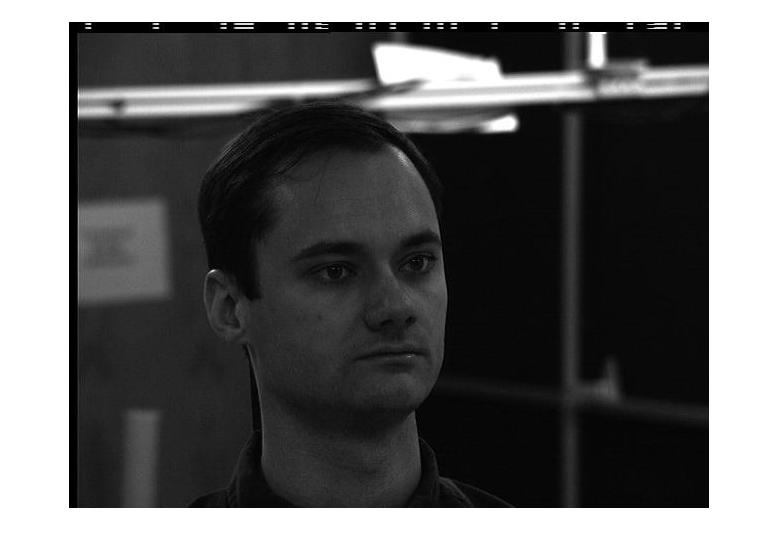
\includegraphics[width=50mm]{figure/02-1-1-o}
    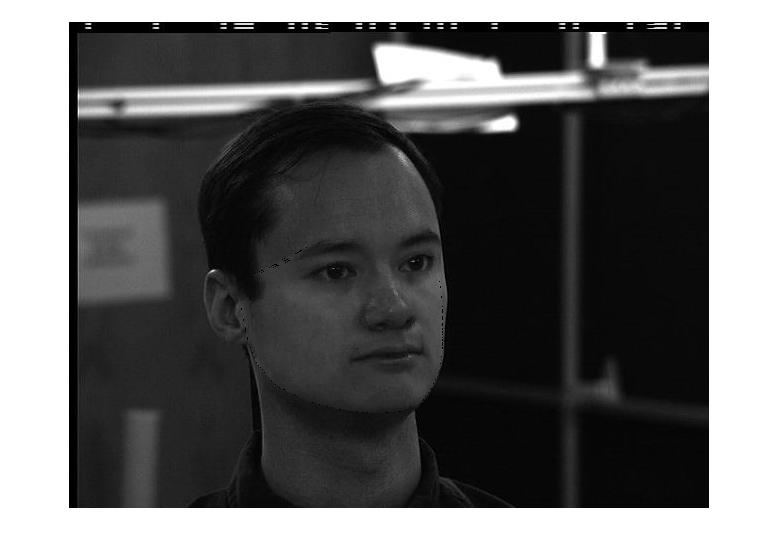
\includegraphics[width=50mm]{figure/02-1-1.jpg}
    
    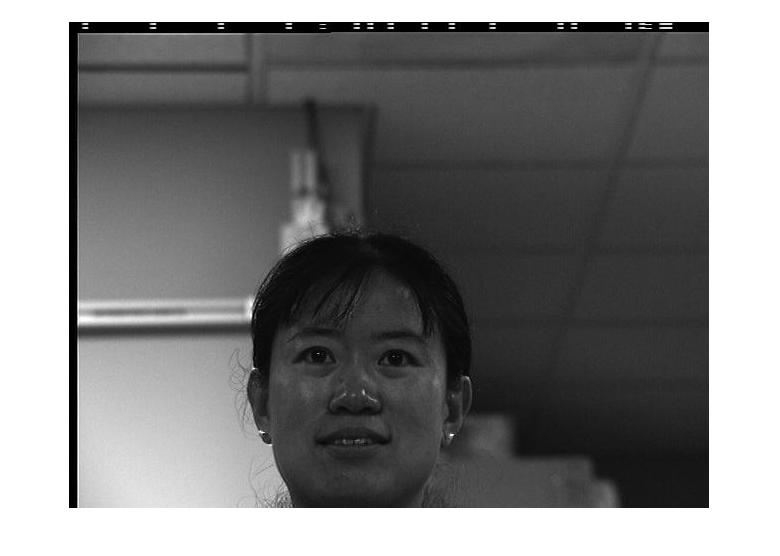
\includegraphics[width=50mm]{figure/01-2-2-o.jpg}
    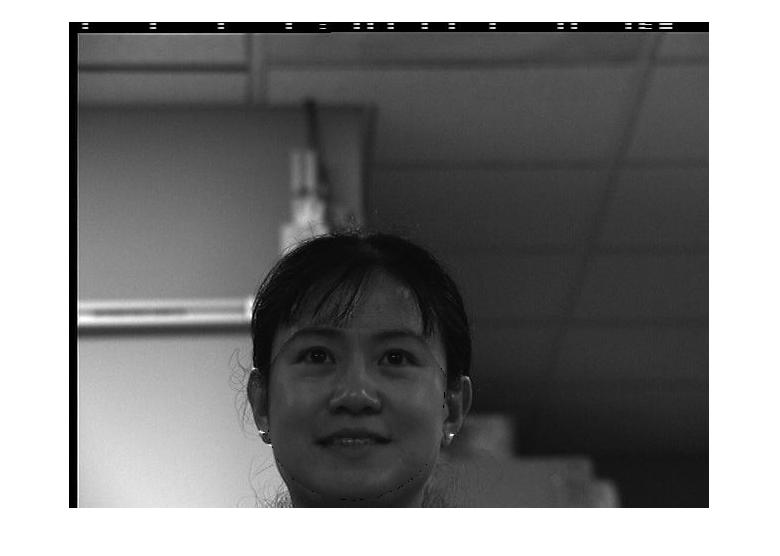
\includegraphics[width=50mm]{figure/01-2-2.jpg}

    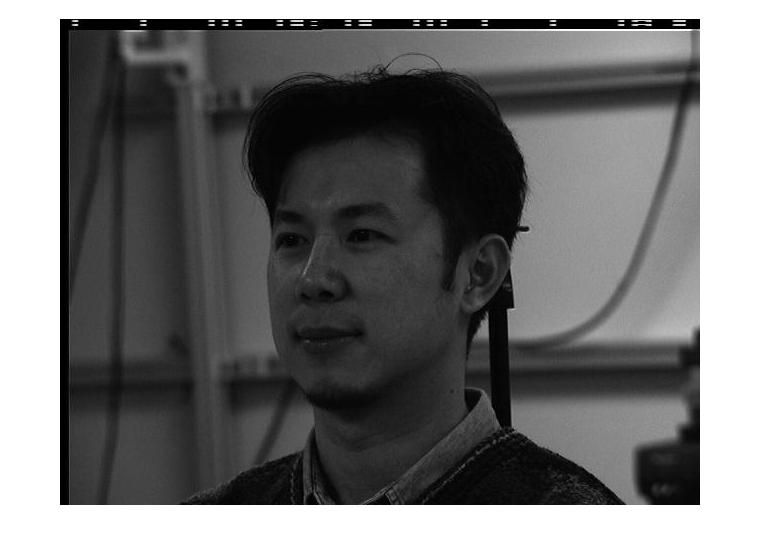
\includegraphics[width=50mm]{figure/59-SW07-o.jpg}
    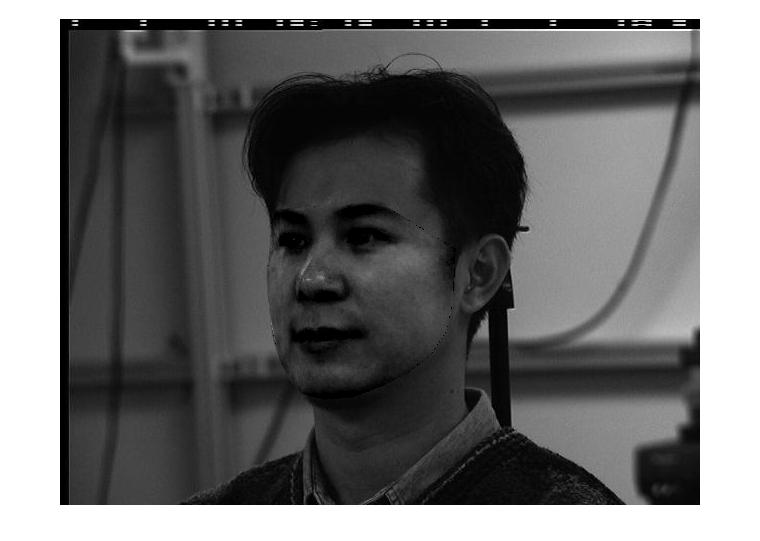
\includegraphics[width=50mm]{figure/59-SW07.jpg}
    \caption{Images comparison for various poses and expressions. Left column: original 
            images. Right column: de-identified results.}
    \label{fig:app_comparison}
\end{figure}

To show the flexibility of proposed approach, we conduct another experiment on IMM dataset. A
tensor is constructed based on two factors: {\it identity, illumination}. 35 persons are chosen.
Each of them has two images under different illuminations. The other images are for testing.
With a similar process as in CMU PIE, we get the de-identified images in IMM. Figure 
\ref{fig:light_comparison} is one example. 

Observing the Fig. \ref{fig:app_comparison} and Fig. \ref{fig:light_comparison}, the proposed
algorithm could produce visual natrual de-identified images and could preserve {\it data utility}. 

\begin{figure}[!htb]
    \centering
    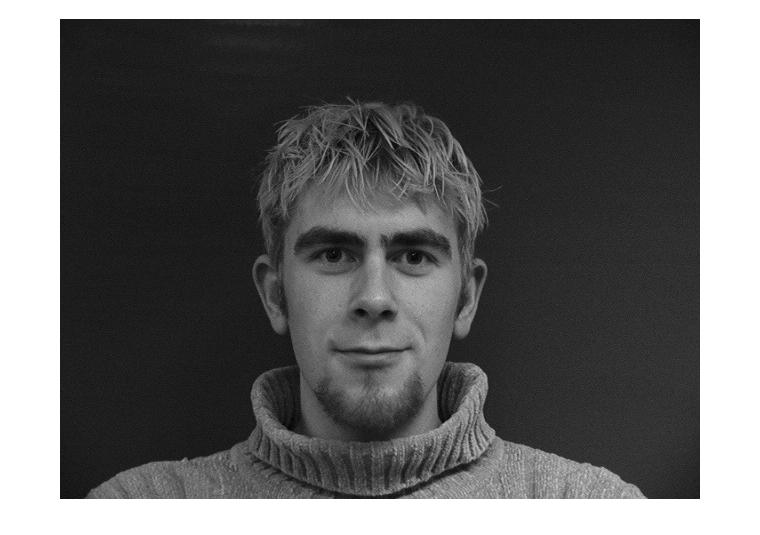
\includegraphics[width=50mm]{figure/IMM_nolight_o}
    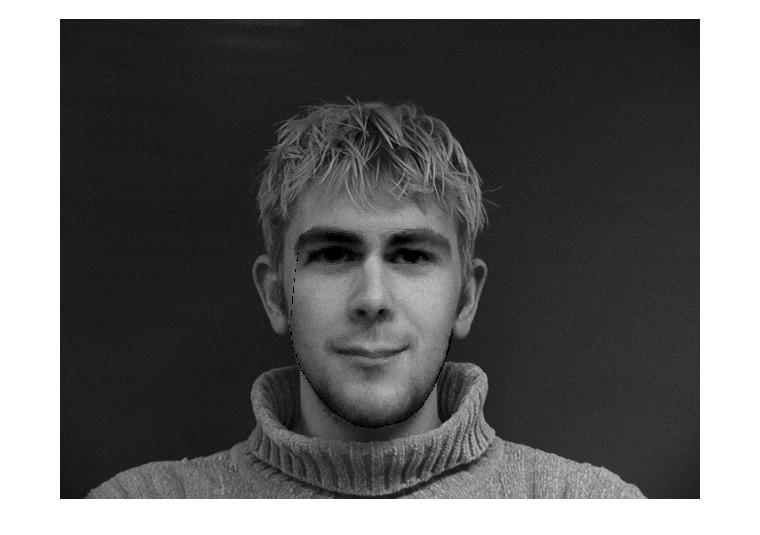
\includegraphics[width=50mm]{figure/IMM_nolight_d}

    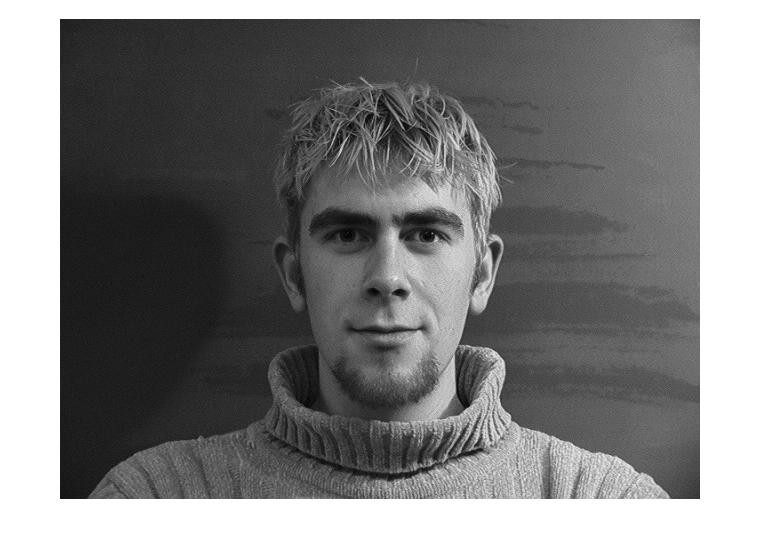
\includegraphics[width=50mm]{figure/IMM_light_o}
    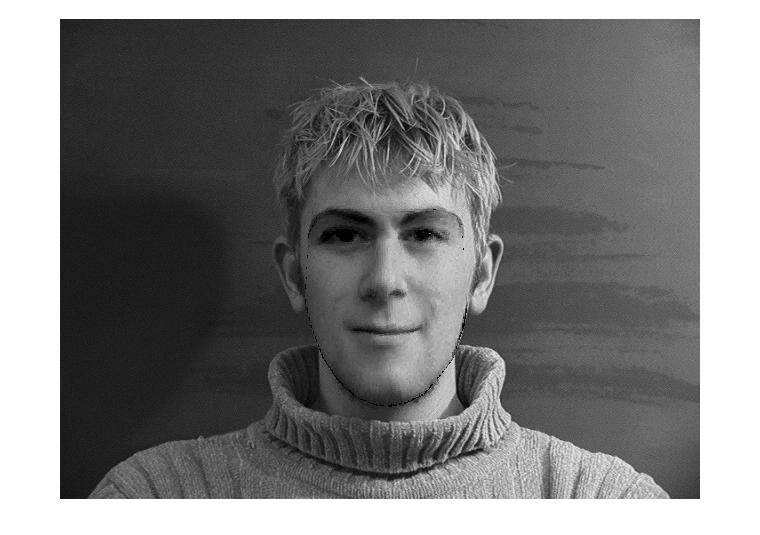
\includegraphics[width=50mm]{figure/IMM_light_d}
    
    \caption{Images comparison for various illuminations. Left column: original 
            images. Right column: de-identified results.}
    \label{fig:light_comparison}
\end{figure}


\subsection{Face Recognition and Expression Recognition}

  Except for visual effect, the proposed algorithm should also be verified by automatic recognition
  algorithms. Using the de-identified results of CMU PIE, we test the quality of privacy protection by face
  recognition algorithms and test the quality of data utility preservation by expression recognition algorithms. 
  

  For identity information, one of the best face recognizers, FaceNet \cite{facenet15} and it opensource 
  implementation \cite{openface16} are used to test the data before and after de-identification. For expression, 
  a general framework, PCA+SVM, is used. If the de-identified results could baffle the best face recognizer and 
  can be figured out clearly by a common expression recognizer, the de-identification algorithm is convincible. 
    \begin{table}[ht]
        \begin{center}
        \begin{tabular}{|c|c|c|}    % 62.5\%, 42.5\%, 35.83\%, 35\%
            \hline
            State               & Face Recognition  & Expression Recognition  \\
            \hline
            Before              & $100\%$       & $100\%$           \\
            \hline
            k = 2               & $52.50\%$       & $100\%$           \\
            \hline
            k = 3             & $37.50\%$       & $100\%$           \\
            \hline
            k = 4             & $31.67\%$    & $100\%$           \\
            \hline
            k = 5             & $26.67\%$     & $100\%$           \\
            \hline
        \end{tabular}
        \end{center}
        \caption{The comparison of face recognition accuracy, expression recognition accuracy 
        before and after de-identification. 'Before' is for original data without 
        de-identification and $k$ is for $k$ images (including the target image) that are used in de-identification.}
    \end{table}

\subsection{Reasons of Using Rank-$r$ Approximation}
    This part explains why we use rank-$r$ approximation rather than rank-1 approximation in
    parameters decomposition. 
    To represent a face image with multiple vector parameters, rank-1 approximation seems to be the best
    algorithm. 
    However, rank-1 approximation easily produces low-quality reconstruction images 
    when some features of the input image never appear in the pre-constructed tensor.
    Rank-$r$ approximation could improve the quality.

    As shown in Figure \ref{fig:glass}, an image with glasses causes ridiculous reconstruction result because
    all the images in pre-constructed tensor are without glasses.

    \begin{figure}[!htb]
      \centering
      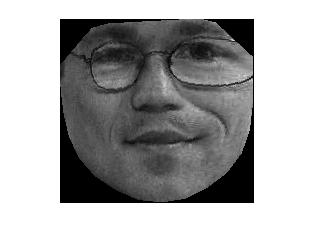
\includegraphics[width=40mm]{figure/untrain}
      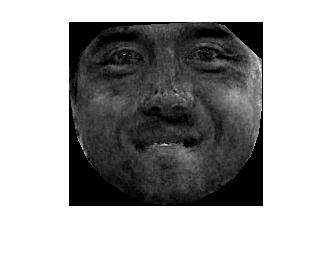
\includegraphics[width=40mm]{figure/untrain-rank1}
      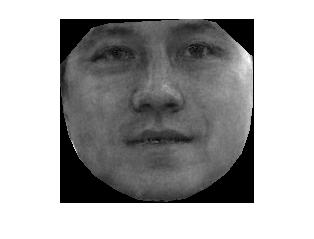
\includegraphics[width=40mm]{figure/untrain-a}

      \caption{Comparison of reconstruction results by rank-1 and rank-$r$ approximation. 
      Left: original image. Middle: rank-1 approximation. Right: rank-$r$ approximation.} %
      \label{fig:glass}
    \end{figure}


    If the features of a image is not included in the pre-constructed tensor, our algorithm
    is not able to recover it. As an analogy, a 3D point loses one dimension data when projecting
    it into a 2D plane. We would use rank-$n$ approximation to reconstruct the data as close as
    possible then de-identify it. 
    Figure \ref{fig:glass_deidentify} 
    shows a de-identification example of our model for an image with new features.
    We use rank-$n$ approximation of a tensor to enlarge 
    the model representation ability.
    \begin{figure}[htb]
      
      \centering  
      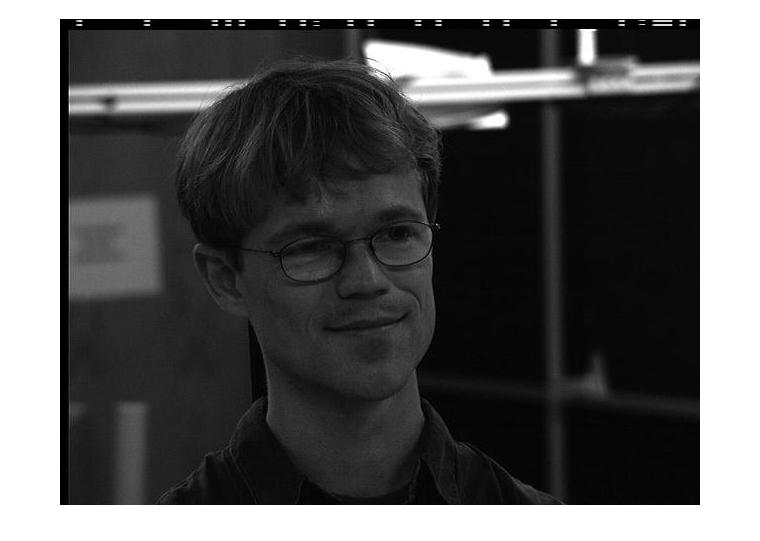
\includegraphics[width=60mm]{figure/61-1-2-o}
      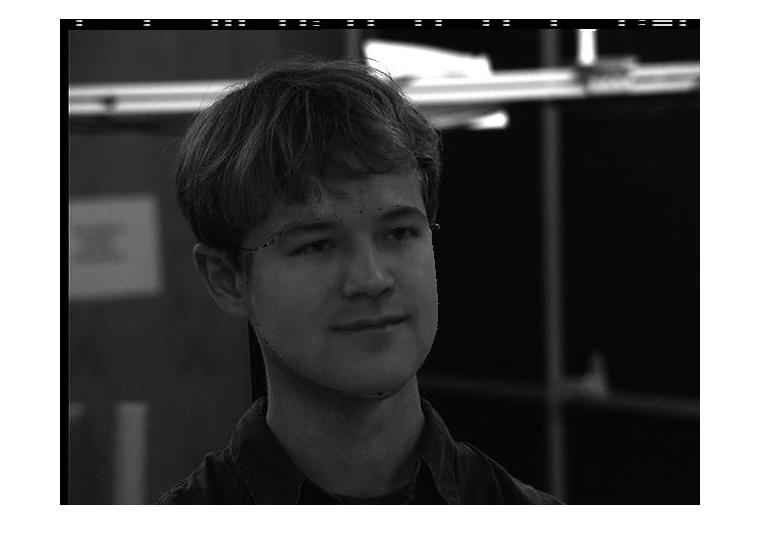
\includegraphics[width=60mm]{figure/61-1-2}

    \caption{De-identification for an image with new features.}
    \label{fig:glass_deidentify}
    \end{figure}

